\documentclass[11pt,a4paper]{article}
\usepackage[margin=2.2cm]{geometry}
\usepackage[T1]{fontenc}
\usepackage{lmodern}
\usepackage{amsmath,amssymb}
\usepackage{graphicx}
\usepackage{booktabs}
\usepackage{float}
\usepackage{xcolor}
\usepackage{listings}
\usepackage[hidelinks]{hyperref}

\graphicspath{{figures/}{handwritten/}}

\lstdefinestyle{rcode}{
  language=R,
  basicstyle=\ttfamily\footnotesize,
  commentstyle=\color{teal!70!black},
  keywordstyle=\color{blue!60!black}\bfseries,
  stringstyle=\color{red!60!black},
  backgroundcolor=\color{gray!6},
  frame=single, rulecolor=\color{gray!40},
  breaklines=true, columns=fullflexible, keepspaces=true,
  showstringspaces=false, upquote=true,
  literate={<-}{{$\leftarrow$}}1
}
\lstdefinestyle{rout}{
  basicstyle=\ttfamily\footnotesize,
  frame=leftline, rulecolor=\color{gray!60},
  breaklines=true, columns=fullflexible, keepspaces=true
}
\lstset{style=rcode}

% one handwritten page, scaled to fit
\newcommand{\handwritten}[2][0.82]{%
  \begin{center}\includegraphics[width=\textwidth,height=#1\textheight,keepaspectratio]{#2}\end{center}}

\title{MATH 4515 -- Assignment 2}
\author{Erik Jin \\ Student ID: \texttt{XXXXXXXX}}
\date{3 November 2026}

\begin{document}
\maketitle

\noindent All simulations are done in R (notebook \texttt{MATH4515\_assignment2.ipynb}, kernel \texttt{ir}); every
code block below is copied from that notebook and is followed by its output. Derivations are handwritten and
included as scans. The helper below is used in Problem~1 and the Bonus problem.

\begin{lstlisting}
library(readxl)

options(repr.plot.width = 10, repr.plot.height = 4, scipen = 10)

# Monte Carlo table: for each n in num_sim, draw n values of Y with sim_Y(n) and
# report the estimate mean(Y), SE = sd(Y)/sqrt(n) and PE = SE/estimate.
mc_table <- function(sim_Y, num_sim) {
    estimates <- numeric(length(num_sim))
    standard_errors <- numeric(length(num_sim))
    for (i in seq_along(num_sim)) {
        Y <- sim_Y(num_sim[i])
        estimates[i] <- mean(Y)
        standard_errors[i] <- sd(Y) / sqrt(num_sim[i])
    }
    p_errors <- standard_errors / estimates
    data.frame(
        n        = format(num_sim, scientific = FALSE, big.mark = ","),
        estimate = signif(estimates, 6),
        SE       = signif(standard_errors, 4),
        PE       = sprintf("%.3f%%", p_errors * 100)
    )
}
\end{lstlisting}

% =====================================================================
\section*{Problem 1 -- Monte Carlo estimation}

Each quantity is written as $\mathbb{E}[Y]$ for a suitable $Y$ and estimated by the sample mean of $n$ simulated
values. The accuracy is measured by
\[
  SE = \frac{s_Y}{\sqrt n}, \qquad PE = \frac{SE}{\bar Y},
\]
and $PE < 0.5\%$ requires
\[
  \frac{s_Y}{\sqrt n\,\bar Y} < 0.005 \iff n > \left(\frac{\sigma_Y}{0.005\,\mu_Y}\right)^2 .
\]
For every part the simulation is run for $n = 10^4, \dots, 10^7$ and the required $n$ is computed either
exactly or from a pilot run.

\subsection*{(a) $\mathbb{E}[X^4]$, $X \sim N(0,1)$}

Here $Y = X^4$. Since $\mathbb{E}[X^4] = 3$ and $\mathbb{E}[X^8] = 105$, $\operatorname{Var}(Y) = 96$ and
$n > 96/(0.005\cdot 3)^2 \approx 426\,667$.

\begin{lstlisting}
# Y = X^4. Theory: E[X^4] = 3 and Var(X^4) = E[X^8] - 9 = 105 - 9 = 96,
# so PE < 0.5% requires n > 96 / (0.005 * 3)^2 = 426,667.
set.seed(0)
num_sim <- c(1e4, 1e5, 1e6, 1e7)
sim_a <- function(n) rnorm(n, mean = 0, sd = 1)^4
mc_table(sim_a, num_sim)
96 / (0.005 * 3)^2    # theoretical number of runs needed
\end{lstlisting}
\begin{lstlisting}[style=rout]
  n          estimate SE       PE    
1     10,000 2.86398  0.086790 3.030%
2    100,000 3.01901  0.031200 1.034%
3  1,000,000 3.00612  0.009797 0.326%
4 10,000,000 3.00088  0.003091 0.103%
[1] 426666.7
\end{lstlisting}

\noindent With $n = 10^6$ and $10^7$ the percentage error is below $0.5\%$, in line with the theoretical bound.
\textbf{Answer:} $\mathbb{E}[X^4] \approx 3.0009$ ($n = 10^7$, $PE = 0.103\%$); the exact value is $3$.

\subsection*{(b) $\mathbb{E}[\min(\max(X - 1000, 0), 6000)]$, $X \sim \text{Gamma}(\alpha = 3.6,\ \theta = 1000)$}

$X$ is drawn with \texttt{rgamma(n, shape = 3.6, scale = 1000)} and $Y$ is computed elementwise with
\texttt{pmin}/\texttt{pmax}. $\operatorname{Var}(Y)$ is not available in closed form, so a pilot run of $10^5$
gives $s_Y$ and $\bar Y$, and the required $n$ is about $17\,500$.

\begin{lstlisting}
# Y = min(max(X - 1000, 0), 6000) elementwise (pmin/pmax), X drawn with rgamma (scale = theta).
set.seed(0)
alpha <- 3.6
theta <- 1000
sim_b <- function(n) pmin(pmax(rgamma(n, shape = alpha, scale = theta) - 1000, 0), 6000)
mc_table(sim_b, num_sim)

# Pilot run to find the required n: n > (s_Y / (0.005 * mean_Y))^2
Y_pilot <- sim_b(1e5)
(sd(Y_pilot) / (0.005 * mean(Y_pilot)))^2
\end{lstlisting}
\begin{lstlisting}[style=rout]
  n          estimate SE      PE    
1     10,000 2531.99  16.7800 0.663%
2    100,000 2525.03   5.2910 0.210%
3  1,000,000 2528.42   1.6770 0.066%
4 10,000,000 2529.39   0.5299 0.021%
[1] 17482.86
\end{lstlisting}

\noindent\textbf{Answer:} $\mathbb{E}[\min(\max(X - 1000, 0), 6000)] \approx 2529.4$ ($n = 10^7$, $PE = 0.021\%$).

\subsection*{(c) $P(X_1 + X_2 + X_3 > 9)$, $X_i$ i.i.d.\ general $t$ with $\mu = 1$, $\lambda = 1$, $\nu = 3.5$}

A general $t$ variable is $X = \mu + \lambda T$ with $T \sim t_\nu$, so $X_i$ is generated by
\texttt{mu + lambda * rt(n, df)}. The probability is the mean of the indicator
$I = \mathbf 1\{X_1 + X_2 + X_3 > 9\}$, for which $s_I/\sqrt n = \sqrt{\hat p(1-\hat p)/n}$. Hence
$PE < 0.5\%$ requires $n > \frac{1-p}{p\,(0.005)^2} \approx 2.6\times 10^6$; a small probability needs many runs.

\begin{lstlisting}
# X_i = mu + lambda * T_i with T_i ~ t(df). Each row of the n x 3 matrix is one run (X1, X2, X3).
# The probability is the mean of the indicator I = 1{X1 + X2 + X3 > 9}, so
# sd(I)/sqrt(n) = sqrt(p(1 - p)/n) and PE < 0.5% requires n > (1 - p) / (p * 0.005^2).
set.seed(0)
mu <- 1
lambda <- 1
df <- 3.5
sim_c <- function(n) {
    X <- matrix(mu + lambda * rt(3 * n, df), ncol = 3)
    as.numeric(rowSums(X) > 9)
}
mc_table(sim_c, num_sim)

p_pilot <- mean(sim_c(1e6))
(1 - p_pilot) / (p_pilot * 0.005^2)    # required n
\end{lstlisting}
\begin{lstlisting}[style=rout]
  n          estimate  SE         PE    
1     10,000 0.0153000 0.00122700 8.023%
2    100,000 0.0152900 0.00038800 2.538%
3  1,000,000 0.0152290 0.00012250 0.804%
4 10,000,000 0.0150224 0.00003847 0.256%
[1] 2604628
\end{lstlisting}

\noindent\textbf{Answer:} $P(X_1 + X_2 + X_3 > 9) \approx 0.01502$ ($n = 10^7$, $PE = 0.256\%$).

% =====================================================================
\section*{Problem 2 -- Generating random numbers}

Each generator \texttt{r...(n)} returns $n$ draws, like \texttt{rnorm(n)}. To check each algorithm, the histogram
of $100\,000$ draws is compared with the target density (red curve).

\subsection*{(a) Inverse transformation}

\handwritten{IMG_4391.jpg}

\begin{lstlisting}
# F(x) = 1 - exp(-x^3/3)  =>  X = F^{-1}(U) = (-3 log(1 - U))^(1/3)
F_inv_a <- function(U) {
    X <- (-3 * log(1 - U))^(1 / 3)
    return(X)
}
rX_a <- function(n) F_inv_a(runif(n))

set.seed(1)
X_a <- rX_a(100000)
hist(X_a, breaks = 100, freq = FALSE, col = "grey", main = "Problem 2(a)", xlab = "x")
curve(x^2 * exp(-x^3 / 3), add = TRUE, col = "red", lwd = 2)
\end{lstlisting}

\begin{figure}[H]
  \centering
  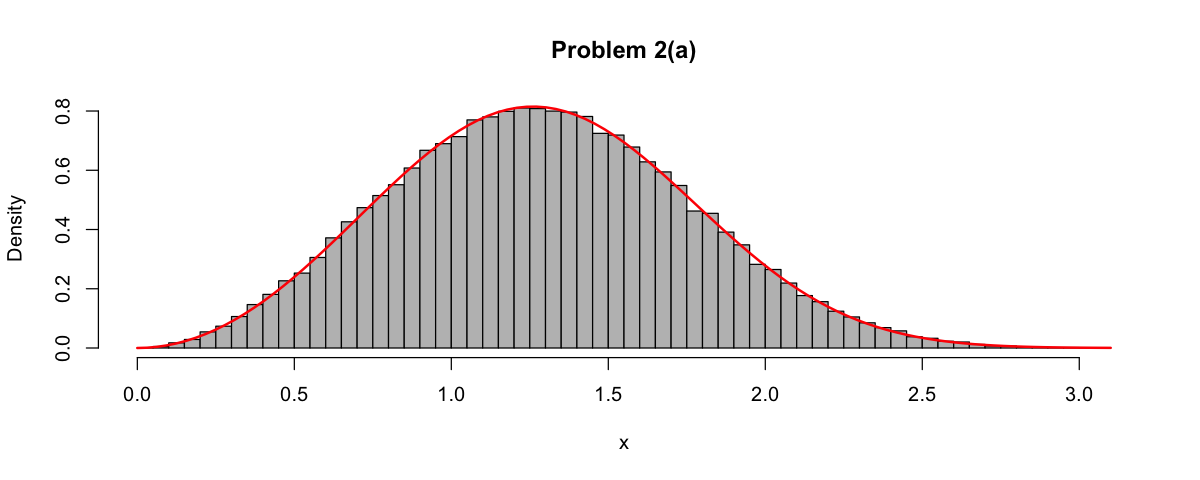
\includegraphics[width=0.85\textwidth]{p2a_hist.png}
  \caption{$100\,000$ draws from $f_X(x) = x^2 e^{-x^3/3}$ with the inverse transform.}
\end{figure}

\subsection*{(b) Discrete inverse transformation}

\handwritten{IMG_4392.jpg}

\begin{lstlisting}
# sum_{k>=1} C/k! = C(e - 1) = 0.4  =>  C = 0.4 / (e - 1).
# N = smallest k with F(k) >= U; N is unbounded, so we step through k with a while loop.
C <- 0.4 / (exp(1) - 1)
F_inv_b <- function(u) {
    k <- 0
    Fk <- 0.6                       # F(0) = P(N = 0)
    while (u > Fk) {
        k <- k + 1
        Fk <- Fk + C / factorial(k) # F(k) = F(k - 1) + P(N = k)
    }
    return(k)
}
rN <- function(n) sapply(runif(n), F_inv_b)   # F_inv_b works on one u at a time

set.seed(1)
N <- rN(100000)
k <- 0:5
data.frame(k = k,
           empirical   = round(as.numeric(table(factor(N, levels = k))) / length(N), 4),
           theoretical = round(c(0.6, C / factorial(k[-1])), 4))
\end{lstlisting}
\begin{lstlisting}[style=rout]
  k empirical theoretical
1 0 0.5997    0.6000     
2 1 0.2334    0.2328     
3 2 0.1157    0.1164     
4 3 0.0387    0.0388     
5 4 0.0103    0.0097     
6 5 0.0019    0.0019
\end{lstlisting}

\noindent The empirical frequencies agree with $P(N = k)$ to within simulation noise.

\subsection*{(c) Rejection sampling}

\handwritten{IMG_4393.jpg}
\handwritten{IMG_4394.jpg}
\handwritten[0.4]{IMG_4395.jpg}

\begin{lstlisting}
# Proposal g(y) = 5/(1 + y)^6 with G^{-1}(U) = (1 - U)^(-1/5) - 1.
# M = sup f*/g = 32/5 at y = 1, where f* = f without C; C cancels in the threshold f*/(M g).
g <- function(x) 5 / (1 + x)^6
f_star <- function(x) 1 / (1 + x^6)

rg <- function(n) {             # draws from g by inverse transform
    U <- runif(n)
    X <- (1 - U)^(-1 / 5) - 1
    return(X)
}
M <- 32 / 5
rY <- function(n) {
    Y <- numeric(n)
    i <- 1
    while (i <= n) {
        x <- rg(1)              # X* from g
        u <- runif(1)           # Y* from U(0, 1)
        if (u <= f_star(x) / (M * g(x))) {   # accept X*
            Y[i] <- x
            i <- i + 1
        }
    }
    return(Y)
}

set.seed(1)
Y_c <- rY(100000)
x_prop <- rg(1e6)               # acceptance rate: theory 1/(C M) with C = 3/pi
c(acceptance = mean(runif(1e6) <= f_star(x_prop) / (M * g(x_prop))), theory = pi / 3 / M)
hist(Y_c, breaks = seq(0, ceiling(max(Y_c)), by = 0.05), freq = FALSE, col = "grey",
     xlim = c(0, 3), main = "Problem 2(c)", xlab = "y")
curve(3 / pi / (1 + x^6), add = TRUE, col = "red", lwd = 2)
\end{lstlisting}
\begin{lstlisting}[style=rout]
acceptance     theory 
 0.1637490  0.1636246
\end{lstlisting}

\noindent Since $\int_0^\infty \frac{dy}{1+y^6} = \frac{\pi}{3}$, the normalizing constant is $C = 3/\pi$. It is
not needed by the algorithm, but it gives the theoretical acceptance rate $1/(CM) = \pi/(3M) \approx 0.164$,
which matches the simulation, and the red curve in the figure below.

\begin{figure}[H]
  \centering
  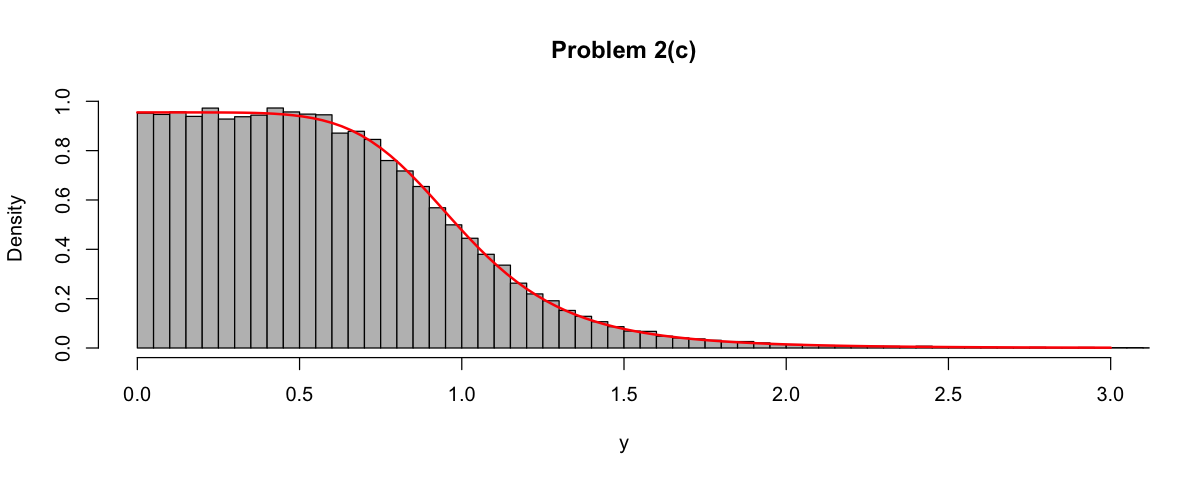
\includegraphics[width=0.85\textwidth]{p2c_hist.png}
  \caption{$100\,000$ draws from $f_Y(y) = C/(1+y^6)$ with rejection sampling (curve: $C = 3/\pi$).}
\end{figure}

% =====================================================================
\section*{Problem 3 -- MLE and bootstrapping}

\handwritten{IMG_4417.jpg}
\handwritten[0.45]{IMG_4418.jpg}

\subsection*{(a)(i) MLE of $\alpha$}

The log-likelihood $\ell(\alpha) = n\log\alpha - (\alpha+1)\sum_i \log x_i$ has
$\ell'(\alpha) = n/\alpha - \sum_i \log x_i = 0$ and $\ell''(\alpha) = -n/\alpha^2 < 0$, so
$\hat\alpha = n / \sum_i \log x_i$ is the maximum.

\begin{lstlisting}
# l(alpha) = n log(alpha) - (alpha + 1) sum(log x_i)  =>  alpha_hat = n / sum(log x_i)
x <- read_excel("MATH4515_HW2_Data1.xlsx")$X
mle_alpha <- function(data) {
    n <- length(data)
    alpha <- n / sum(log(data))
    return(alpha)
}
alpha_hat <- mle_alpha(x)
c(n = length(x), alpha_hat = alpha_hat)
\end{lstlisting}
\begin{lstlisting}[style=rout]
        n alpha_hat 
1560.0000    4.3516
\end{lstlisting}

\noindent\textbf{Answer:} $\hat\alpha = 4.3516$ ($n = 1560$).

\subsection*{(a)(ii) Bootstrap estimate of the MSE}

Draw $B = 10\,000$ resamples of size $n$ with replacement from the data, compute the MLE $\hat\alpha^*_b$ on
each and estimate
\[
  \widehat{\text{MSE}}(\hat\alpha) = \frac1B \sum_{b=1}^B \left(\hat\alpha^*_b - \hat\alpha\right)^2 .
\]

\begin{lstlisting}
# MSE ~= (1/B) sum_b (alpha*_b - alpha_hat)^2, alpha*_b = MLE on a resample of size n with replacement
set.seed(0)
B <- 10000
mle_estimates <- numeric(B)
for (i in 1:B) {
    bootstrap <- sample(x, length(x), replace = TRUE)
    mle_estimates[i] <- mle_alpha(bootstrap)
}
MSE <- mean((mle_estimates - alpha_hat)^2)
c(MSE = MSE, variance = var(mle_estimates), bias = mean(mle_estimates) - alpha_hat)
\end{lstlisting}
\begin{lstlisting}[style=rout]
       MSE   variance       bias 
0.01177734 0.01177512 0.00184125
\end{lstlisting}

\noindent\textbf{Answer:} $\widehat{\text{MSE}} \approx 0.0118$. The bias is only about $0.002$, so the MSE is
almost entirely variance; it agrees with the asymptotic variance $\hat\alpha^2/n \approx 0.0121$.

\subsection*{(b) 98\% confidence interval for $\mu$}

$\mu$ is the (unknown) population mean of the daily log-return and $\bar X$ its estimate. The Shapiro--Wilk test
rejects normality of the returns ($p \approx 2\times 10^{-11}$), so
$T = \frac{\bar X - \mu}{s/\sqrt n}$ need not follow a $t_{n-1}$ distribution. Its distribution is approximated by
the bootstrap-$t$ method (handwritten above):
\[
  T^*_b = \frac{\bar X^*_b - \bar X}{s^*_b/\sqrt n}, \quad b = 1,\dots,B, \qquad
  t_L = 1\%\text{ quantile}, \ t_U = 99\%\text{ quantile of } T^*,
\]
\[
  98\% \approx P\!\left(t_L \le \frac{\bar X - \mu}{s/\sqrt n} \le t_U\right)
  = P\!\left(\bar X - t_U\frac{s}{\sqrt n} \le \mu \le \bar X - t_L\frac{s}{\sqrt n}\right).
\]
The first observation has no log-return and is removed, which leaves $n = 1004$. The resampling assumes
i.i.d.\ observations, and $n$ is large enough for the bootstrap distribution to approximate the distribution of $T$.

\begin{lstlisting}
# Bootstrap-t: the distribution of T = (Xbar - mu)/(s/sqrt(n)) is approximated by the B values of
# T* = (Xbar* - Xbar)/(s*/sqrt(n)). With t_L, t_U the 1% and 99% quantiles of T*:
# CI = [Xbar - t_U s/sqrt(n), Xbar - t_L s/sqrt(n)]
set.seed(0)
data <- read_excel("MATH4515_HW2_Data2.xlsx")
data <- na.omit(data)          # the first day has no log-return
returns <- data$`Stock A`
B <- 10000
n <- length(returns)
t_stats <- numeric(B)
x_mean <- mean(returns)
x_std <- sd(returns)
for (i in 1:B) {
    b_sample <- sample(returns, size = n, replace = TRUE)
    b_mean <- mean(b_sample)
    b_s <- sd(b_sample)
    t_stats[i] <- (b_mean - x_mean) / (b_s / sqrt(n))
}
t_l <- unname(quantile(t_stats, 0.01))
t_u <- unname(quantile(t_stats, 0.99))
CI_mu <- c(x_mean - x_std / sqrt(n) * t_u, x_mean - x_std / sqrt(n) * t_l)
c(n = n, x_mean = x_mean, s = x_std)
c(t_l = t_l, t_u = t_u)
c(CI_lower = CI_mu[1], CI_upper = CI_mu[2])

format(shapiro.test(returns)$p.value, scientific = TRUE, digits = 3)  # normality is rejected, which motivates the bootstrap
hist(t_stats, breaks = 100, freq = FALSE, col = "grey", main = "Bootstrap distribution of T*", xlab = "T*")
curve(dt(x, df = n - 1), add = TRUE, col = "red", lwd = 2)
\end{lstlisting}
\begin{lstlisting}[style=rout]
             n         x_mean              s 
1004.000000000    0.003167057    0.029625407
      t_l       t_u 
-2.310684  2.329909
   CI_lower    CI_upper 
0.000988663 0.005327476
[1] "1.78e-11"
\end{lstlisting}

\begin{figure}[H]
  \centering
  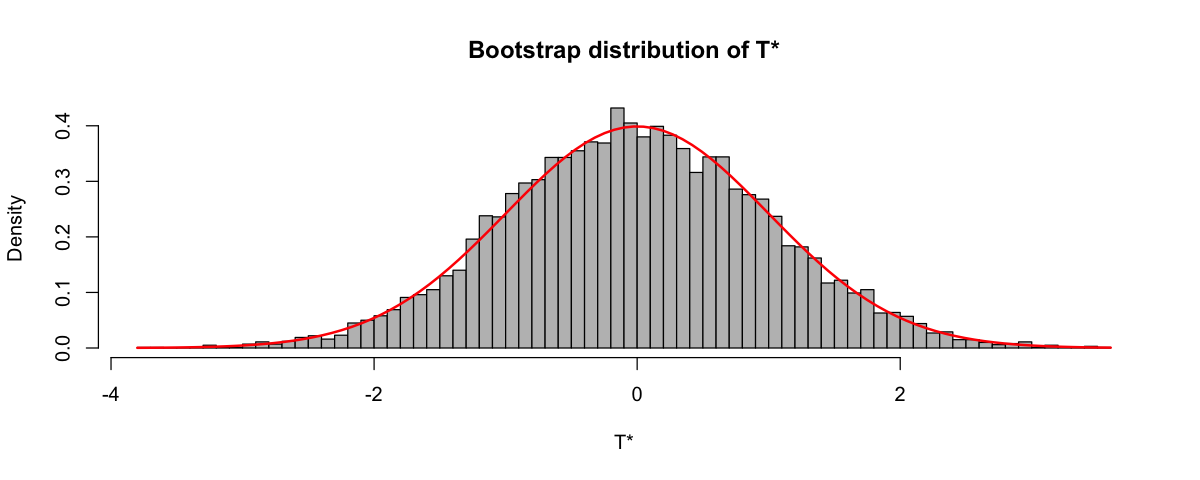
\includegraphics[width=0.85\textwidth]{p3b_tstar.png}
  \caption{Bootstrap distribution of $T^*$ ($B = 10\,000$) with the $t_{n-1}$ density for comparison.}
\end{figure}

\noindent\textbf{Answer:} the 98\% confidence interval is
$\mu \in [\,0.000989,\ 0.005327\,]$. The interval lies entirely above $0$, so the average daily log-return
is significantly positive at the 2\% level. With $n = 1004$ it is close to the $t$-interval, but it does
not rely on normality.

% =====================================================================
\section*{Bonus Problem}

\handwritten{IMG_4419.jpg}
\handwritten[0.3]{IMG_4420.jpg}

\subsection*{(a) $\mathbb{E}[\max(4800 - 140X - X^2, 0)]$, $X \sim N(10, 100)$}

Here $Y = \max(4800 - 140X - X^2, 0)$ is computed elementwise with \texttt{pmax}. The number of runs is
chosen as in Problem 1 by increasing $n$ until $PE < 0.5\%$.

\begin{lstlisting}
set.seed(0)
mu <- 10
std <- sqrt(100)
num_sim <- c(1e3, 1e4, 1e5, 1e6, 1e7)
sim_bonus <- function(n) {
    x <- rnorm(n, mean = mu, sd = std)
    pmax(4800 - 140 * x - x^2, 0)
}
mc_table(sim_bonus, num_sim)
\end{lstlisting}
\begin{lstlisting}[style=rout]
  n          estimate SE      PE    
1      1,000 3250.47  48.8900 1.504%
2     10,000 3207.81  15.4400 0.481%
3    100,000 3225.63   4.8750 0.151%
4  1,000,000 3226.29   1.5420 0.048%
5 10,000,000 3226.61   0.4875 0.015%
\end{lstlisting}

\noindent $n = 10^4$ is just below the limit ($0.481\%$), so $n = 10^5$ is chosen to have a margin
($PE = 0.151\%$). \textbf{Answer:} $\mathbb{E}[\max(4800 - 140X - X^2, 0)] \approx 3226$.

\subsection*{(b) Distribution of $Y = X_1 + X_2 + X_3$}

Each $X_i$ is drawn by rejection sampling with the proposal $g(x) = e^{-x}$ and
$M = e^{x_0 - x_0^4} \approx 1.604$, $x_0 = (1/4)^{1/3}$ (handwritten above); $C$ cancels in the threshold. The
rejection step is vectorised: proposals are generated in batches and the accepted ones are kept until $3n$
draws are available, which are arranged as an $n \times 3$ matrix whose row sums are $n$ draws of $Y$.

\begin{lstlisting}
# Proposal g(x) = e^{-x} (Exp(1)) with G^{-1}(U) = -log(1 - U).
# f*/g = exp(x - x^4) is maximal at x0 = (1/4)^(1/3), so M = exp(x0 - x0^4) ~= 1.604; C cancels.
rg_exp <- function(n) {
    U <- runif(n)
    X <- -log(1 - U)
    return(X)
}
f_star_x <- function(x) exp(-x^4)
g_x <- function(x) exp(-x)
x0 <- (1 / 4)^(1 / 3)
M_x <- exp(x0 - x0^4)

# Vectorised rejection: propose in batches and keep the accepted draws until we have n of them
rX <- function(n) {
    X <- numeric(0)
    while (length(X) < n) {
        x <- rg_exp(n)
        u <- runif(n)
        X <- c(X, x[u <= f_star_x(x) / (M_x * g_x(x))])
    }
    return(X[1:n])
}
rY_sum <- function(n) rowSums(matrix(rX(3 * n), ncol = 3))   # each row is (X1, X2, X3)

set.seed(0)
par(mfrow = c(1, 3))
for (n in c(1e3, 1e4, 1e6)) {
    Y <- rY_sum(n)
    hist(Y, breaks = 100, freq = FALSE, col = "grey",
         main = paste("n =", format(n, big.mark = ",", scientific = FALSE)), xlab = "Y")
}
par(mfrow = c(1, 1))

# Y now holds the n = 1,000,000 sample. Check: E[Y] = 3 E[X] = 3 Gamma(1/2) / (4 Gamma(5/4))
c(M = M_x, mean_Y = mean(Y), theory = 3 * gamma(1 / 2) / (4 * gamma(5 / 4)), sd_Y = sd(Y))
quantile(Y, c(0.01, 0.05, 0.5, 0.95, 0.99))
\end{lstlisting}
\begin{lstlisting}[style=rout]
        M    mean_Y    theory      sd_Y 
1.6039517 1.4669266 1.4666116 0.5450962
       1%        5%       50%       95%       99% 
0.3540508 0.6085640 1.4426615 2.4057601 2.8058793
\end{lstlisting}

\begin{figure}[H]
  \centering
  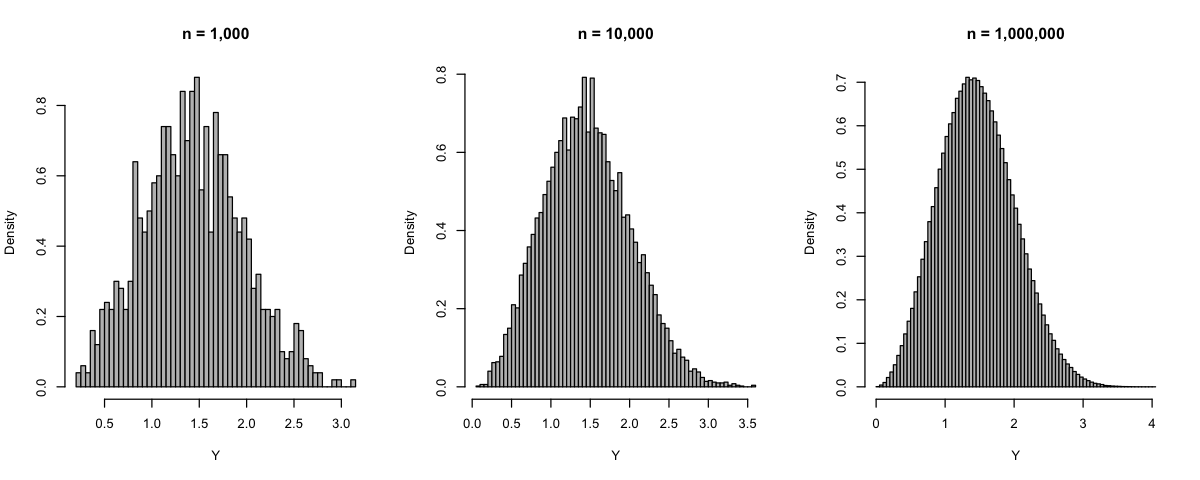
\includegraphics[width=\textwidth]{bonus_b_hist.png}
  \caption{Histogram of $Y = X_1 + X_2 + X_3$ for increasing numbers of simulation runs.}
\end{figure}

\noindent With $n = 10^3$ and $10^4$ the histogram is still noisy, while with $n = 10^6$ it is smooth, so
$n = 10^6$ is used. $Y$ is unimodal with mode near $1.4$, slightly right-skewed, and has mean
$\approx 1.467$ (exact: $3\,\Gamma(1/2)/(4\,\Gamma(5/4)) = 1.4666$) and standard deviation $\approx 0.545$.

\end{document}
